\StartChapter[sec:11-unsupervised-learning]{Unsupervised Learning}
\begin{defbox}[Unsupervised Learning]
Lernen ohne vorgegebene \ZSFkeyword*{Labels} bzw.\ \ZSFkeyword*{Zielwerte}. Der Algorithmus erkennt \ZSFkeyword*{Strukturen} nur anhand der Eingabedaten.
\end{defbox}

\SubsectionBar[sec:11-clustering]{Clustering}
\ZSFindex[unuberwachtes-lernen]{Unüberwachtes Lernen}
\ZSFindex{Clustering}

\SubsubsectionBar{K-Means: ähnliche Punkte gruppieren}
\ZSFindex{K-Means}
\begin{defbox}[K-Means]
K-Means ist ein \ZSFkeyword*{unüberwachter Lernalgorithmus}, der $n$ Datenpunkte in $K$ \ZSFkeyword*{disjunkte Cluster} aufteilt, indem die \ZSFkeyword*{Varianz innerhalb der Cluster} (\ZSFkeyword{Intra-Cluster-Varianz}) minimiert wird.
\end{defbox}

\SubsubsectionBar{Zielfunktion}
\begin{contentbox}[Loss Function]
Sei:
\begin{factlist}
\ZSFFact{$X = {\mathbf{x}_1, \dots, \mathbf{x}_n}$}{mit $\mathbf{x}_i \in \R^d$}
\ZSFFact{$\mu_k$}{\ZSFkeyword{Centroid}: Mittelpunkt der Punkte in Cluster $k$ (kein echter Datenpunkt nötig)}
\ZSFFact{$C_k$}{Menge der Punkte im Cluster $k$}
\end{factlist}
\end{contentbox}

\begin{formulabox}
Die \ZSFkeyword{Verlustfunktion} (\ZSFkeyword*{Distortion} bzw.\ \ZSFkeyword*{Inertia}) lautet:

$
J = \sum_{k=1}^{K} \sum_{\mathbf{x}_i \in C_k} \| \mathbf{x}_i - \mu_k \|^2
$

\ZSFkeyword*{Lesen:} Kleine Distortion $=$ kompakte Cluster. \ZSFkeyword*{Ziel:}

$
\min_{C_1,\dots,C_K, \ \mu_1,\dots,\mu_K} J
$
\end{formulabox}

\SubsubsectionBar{Lloyd's Algorithm}
\ZSFindex{Lloyd-Algorithmus}
\begin{procedure}[Standard K-Means]
\ProcStep{Initialisierung}{Wähle $K$ initiale \ZSFkeyword*{Centroide} (zufällig oder \ZSFkeyword{k-means++}).}
\ProcStep{Zuweisung}{Weise jeden Punkt seinem \ZSFkeyword*{nächstgelegenen Centroid} zu.}
\ProcStep{Update}{Setze jeden Centroid auf den \ZSFkeyword*{Mittelwert} seiner zugewiesenen Punkte.}
\ProcStep{Wiederhole}{Schritte 2--3, bis sich die \ZSFkeyword*{Zuweisungen nicht mehr ändern}.}
\ProcStep{Mehrere Starts}{\ZSFkeyword*{verschiedene Initialisierungen} testen, um schlechte \ZSFkeyword*{lokale Optima} zu vermeiden.}
\end{procedure}

\begin{statementbox}[K-Means terminiert immer]
$J$ fällt in jedem Schritt \ZSFkeyword*{monoton} und es gibt nur \ZSFkeyword*{endlich viele mögliche Zuordnungen}, also \ZSFkeyword*{terminiert} der Algorithmus garantiert. Die Initialisierung bestimmt nur, \emph{welches} \ZSFkeyword*{lokale Optimum} erreicht wird — \textbf{nicht}, ob er terminiert.
\end{statementbox}

\begin{contentbox}[Lloyd-Algorithmus]
\begin{center}
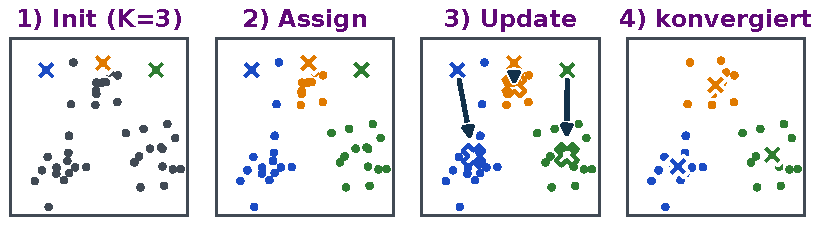
\includegraphics[width=0.74\columnwidth]{Images/kmeans-lloyd-algorithm-iterations.pdf}
\end{center}
\end{contentbox}

\SubsubsectionBar{Elbow-Kriterium: sinnvolles $K$ wählen}
\ZSFindex{Elbow-Kriterium}
\begin{contentbox}
Um $K$ zu wählen, berechne $J(K)$ für verschiedene Werte von $K$ und plotte:
\begin{factlist}
\ZSFFact{x-Achse}{$K$ (\ZSFkeyword*{Anzahl Cluster})}
\ZSFFact{y-Achse}{$J(K)$ (\ZSFkeyword*{Within-Cluster Sum of Squares})}
\end{factlist}
Der \ZSFkeyword*{Elbow-Punkt} ist dort, wo zusätzliche Cluster nur noch \ZSFkeyword*{marginalen Gewinn} bringen — die Kurve macht einen \ZSFkeyword*{sichtbaren Knick}.
\end{contentbox}

\SubsubsectionBar[sec:11-kmeans-code]{K-Means mit scikit-learn}

\begin{propertylist}[Faustregeln]
\ZSFFact{\texttt{n\_clusters} / $K$}{Von dir vorgegebene Anzahl gesuchter Gruppen; mit \ZSFkeyword*{Fachwissen} oder \ZSFkeyword*{Elbow-Kriterium} wählen.}
\ZSFFact{Skalierung}{optional vorher \ZSFkeyword*{skalieren}, wenn Features \ZSFkeyword*{sehr unterschiedliche Grössenordnungen} haben.}
\end{propertylist}

\begin{statementbox}[Merksatz]
\texttt{n\_clusters} legt die \ZSFkeyword*{Anzahl Cluster} fest. Nach \texttt{fit(X)} stehen die \ZSFkeyword*{Zuordnungen} in \texttt{labels\_}.
\end{statementbox}

\begin{codebox}[K-Means: Pflichtschema]
\begin{lstlisting}[style=CodeExpert]
from sklearn.cluster import KMeans
kmeans = KMeans(n_clusters=3, random_state=0)  # ANPASSEN: Anzahl Cluster
kmeans.fit(X)
cluster_labels = kmeans.labels_  # Cluster-IDs (keine Klassenlabels)
\end{lstlisting}
\end{codebox}

\SubsectionBar[sec:11-dimensionsreduktion]{Dimensionsreduktion}
\ZSFindex{Dimensionsreduktion}

\SubsubsectionBar{Grundidee}
\begin{defbox}[Dimensionsreduktion]
Dimensionsreduktionsverfahren stellen \ZSFkeyword*{hochdimensionale Daten} in \ZSFkeyword*{weniger Dimensionen} dar, wobei die wesentliche \ZSFkeyword*{Struktur erhalten bleibt}. Dies erleichtert \ZSFkeyword*{Visualisierung}, \ZSFkeyword*{Rauschunterdrückung} und beschleunigt \ZSFkeyword*{Lernverfahren}.
\end{defbox}

\begin{contentbox}[Feature Selection vs.\ Dimensionsreduktion]
\begin{factlist}
\ZSFFact{Feature Selection}{wählt eine \ZSFkeyword*{Teilmenge der originalen Features} aus; das Ergebnis ist eine \ZSFkeyword*{Teilmenge}.}
\ZSFFact{Dimensionsreduktion}{bildet \ZSFkeyword*{neue Achsen} aus \ZSFkeyword*{Kombinationen der Features} (z.\,B.\ PCA); das Ergebnis sind \ZSFkeyword*{neue Achsen}.}
\end{factlist}
\end{contentbox}

\SubsubsectionBar{PCA (Principal Component Analysis): wichtige Achsen}
\ZSFindex[pca]{PCA / Principal Component Analysis}
\begin{contentbox}
PCA ist ein \ZSFkeyword*{lineares Verfahren}, das neue \ZSFkeyword*{orthogonale Achsen} (\ZSFkeyword{Hauptkomponenten}) bestimmt, entlang derer die \ZSFkeyword*{Varianz der Daten maximal} ist. Die \ZSFkeyword*{erste Hauptkomponente} erfasst die \ZSFkeyword*{grösste Varianz}, die zweite die nächstgrösste, usw. Die Daten werden anschliessend in dieses neue Koordinatensystem \ZSFkeyword*{projiziert}, sodass man von $d$ auf $m \ll d$ Dimensionen reduzieren kann, während der grösste Teil der \ZSFkeyword*{Informationsstreuung} erhalten bleibt.
\end{contentbox}

\SubsubsectionBar{t-SNE: lokale Gruppen sichtbar machen}
\ZSFindex{t-SNE}
\begin{contentbox}
t-SNE ist ein \ZSFkeyword*{nichtlineares Verfahren}, das vor allem \ZSFkeyword*{lokale Nachbarschaften} im Datensatz erhält. Es betont \ZSFkeyword*{kleine Distanzen} und bildet dadurch \ZSFkeyword*{ähnliche Punkte nahe beieinander} ab, was oft zu \ZSFkeyword*{klar getrennten Clustern} in 2D oder 3D führt. Es eignet sich besonders für die \ZSFkeyword*{Visualisierung komplexer Strukturen}.
\end{contentbox}

\SubsubsectionBar[sec:11-dimensionsreduktion-code]{PCA und t-SNE mit scikit-learn}

\begin{propertylist}[Faustregeln]
\ZSFFact{\texttt{n\_components}}{2--3 für \ZSFkeyword*{Visualisierung}; höher, wenn die reduzierten Daten \ZSFkeyword*{weiterverarbeitet} werden.}
\ZSFFact{PCA}{\ZSFkeyword*{linear}, \ZSFkeyword*{schnell} und auf \ZSFkeyword*{maximale Varianz} ausgerichtet.}
\ZSFFact{t-SNE}{\ZSFkeyword*{nichtlinear} und besonders für die \ZSFkeyword*{Visualisierung lokaler Gruppen} geeignet.}
\end{propertylist}

\begin{codebox}[Daten vorbereiten: tabellarisch]
\begin{lstlisting}[style=CodeExpert]
from sklearn.preprocessing import StandardScaler
X = StandardScaler().fit_transform(X)  # OPTIONAL bei unterschiedlichen Skalen
\end{lstlisting}
\end{codebox}

\begin{codebox}[Daten vorbereiten: Bilder]
\begin{lstlisting}[style=CodeExpert]
X = images.reshape(len(images), -1) / 255.0  # flach machen & normieren
\end{lstlisting}
\end{codebox}

\begin{codebox}[PCA: Pflichtschema]
\begin{lstlisting}[style=CodeExpert]
from sklearn.decomposition import PCA
model = PCA(n_components=2)
X_reduced = model.fit_transform(X)
\end{lstlisting}
\end{codebox}

\begin{codebox}[t-SNE: Alternative für Visualisierung]
\begin{lstlisting}[style=CodeExpert]
from sklearn.manifold import TSNE
model = TSNE(n_components=2, random_state=0)
X_reduced = model.fit_transform(X)
\end{lstlisting}
\end{codebox}
